\chapter{NDN~上的游戏设计~NDN Game Design}

\label{gamedesign}


% intro %
% not so sure %
In this section we present game design issues that are specific to NDN games. In most places we use our game adapted from the Unity3D Car Tutorial~\cite{UnityCar} as examples but we are not restricted to this genre.


%-----------------------------------%
\section{P2P Game Architecture}

% why did we choose P2P %
We decided that our sample game should be P2P because of the following reasons. First, P2P architectures are scalable and robust, with minimized network latency (see \ref{game_archi}). Second, these advantages of P2P can be further enhanced by NDN. NDN reduces traffic in the network, which means that given the same bandwidth, more players could join the game. With data packets cached in the network, data receivers will enjoy a even smaller latency. Third, some of the disadvantages of P2P can be (partly) overcame by NDN. Security, for example, will be enhanced by NDN's content validation and trust management scheme. By naming contents instead of hosts, it will be more difficult for attackers to focus on their target. Several types of cheating behavior can be automatically avoided by NDN (see \ref{discussions}). Finally, improvements on P2P architectures will also benefit the hybrid architectures. As an example, the Mirrored Game Server architecture has its clients connected to a local server, but typically orchestrates its distributed servers into a high-performance P2P network, so NDN could positively affect it in a similar way.


%-----------------------------------%
\section{Namespace Design}

% what is a namespace %
Namespace designing is a task specific to NDN application developers. A complete \emph{namespace} of a program is a full collection of names that will be used during the program's execution. Namespace can be presented as trees. For instance, figure~\ref{namespace} is the namespace of our sample car racing game. It is composed of three trees: a \emph{repo tree}, a \emph{network tree} and \emph{game tree}. Each tree node is contains one or more NDN name component(s). One can learn the major functionalities of an application by looking at its namespace design.

\begin{figure}
\begin{center}
\begin{subfigure} [Repo Tree]
{
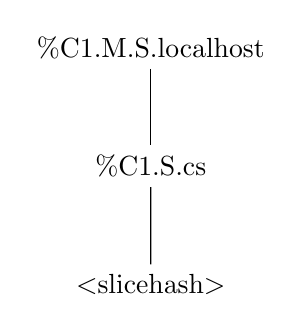
\begin{tikzpicture} [scale=1, transform shape]
    %\tikzstyle{every node}=[rectangle,draw]
    \node {\%C1.M.S.localhost}
        child { node {\%C1.S.cs} 
        		child{ node {$<$slicehash$>$} }
        }
       
    ;
\end{tikzpicture}
\label{repo}
}
\end{subfigure}
\begin{subfigure} [Network Tree]
{
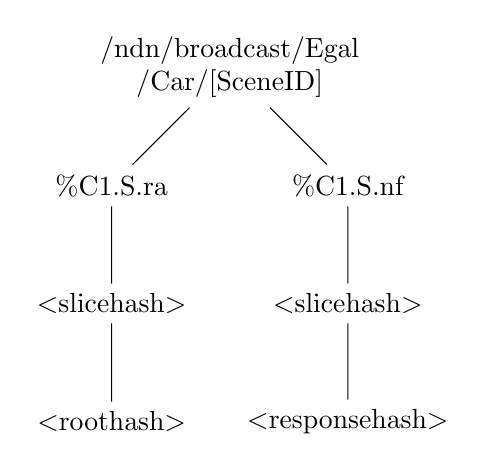
\begin{tikzpicture} [scale=1, transform shape]
    \tikzstyle{every node}=[align = center]
    \tikzstyle{level 1} = [sibling distance=30mm]
    \node {/ndn/broadcast/Egal \\ /Car/[SceneID]}
        child { node {\%C1.S.ra} 
        		child { node {$<$slicehash$>$} 
			child { node {$<$roothash$>$} }
		}
        }
        child { node {\%C1.S.nf}
        		child { node {$<$slicehash$>$} 
			child { node {$<$responsehash$>$} }
		}
        }
    ;
\end{tikzpicture}
\label{broadcast}
}
\end{subfigure}
\begin{subfigure} [Game Tree]
{
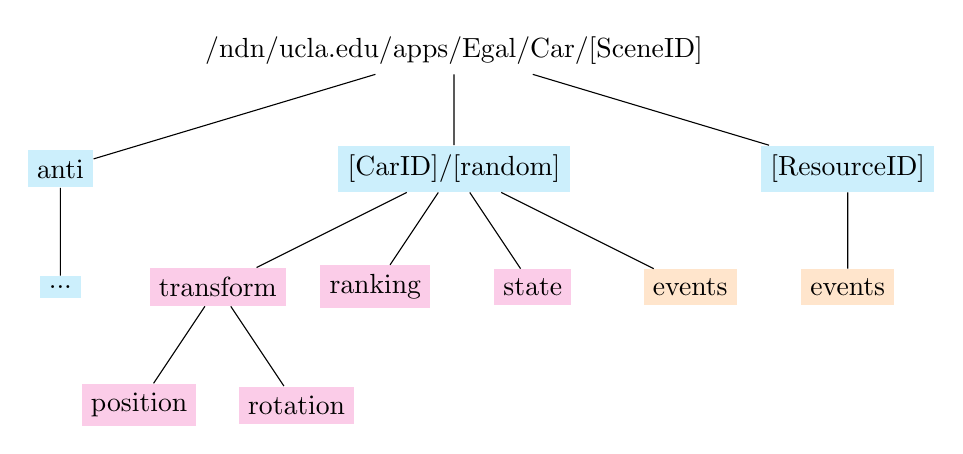
\begin{tikzpicture} [scale=1, transform shape]
    \tikzstyle{every node} = [align=center]
    \tikzstyle{asset} = [fill=cyan!20]
    \tikzstyle{state} = [fill=magenta!20]
    \tikzstyle{event} = [fill=orange!20]
    \tikzstyle{level 1} = [sibling distance=50mm]
    \tikzstyle{level 2} = [sibling distance=20mm]
    \node {/ndn/ucla.edu/apps/Egal/Car/[SceneID]}
        child{ node [asset] {anti}
        		child { node [asset] {...}}
        }
        child { node [asset] { [CarID]/[random]} 
		child { node [state] {transform} 
			child{ node [state] {position} }
			child{ node [state] {rotation} }
		}
		child { node [state] {ranking} }
		child { node [state] {state} }
		child { node [event] {events} }
        } 
         child { node [asset] {[ResourceID]}
        		child {node [event] {events}} }
        
    ;
\end{tikzpicture}
\label{game}
}
\end{subfigure}
\caption[Caption for LOF]{Namespace of our sample car racing game\footnotemark}
\label{namespace}
\end{center}
\end{figure}
\footnotetext{Colors of the nodes will be explained in \ref{ase}. Nodes surrounded by $< >$ will be generated at run time using algorithms chosen by NDN. Nodes surrounded by $[ ]$ are variables that will be substituted with multiple values. Note that \slash~are not part of NDN names, they are for illustration purpose only.}


% localhost namespace: repo %
Names in the Repo Tree are used for communication with the local repository: we use CCNx Create Collection Protocol to create a slice, which is a collection of content objects with a common name prefix. Two parameters are used to define the slice: \emph{topo} and \emph{prefix}. They later become the root node of the network tree and the game tree. \url{\%C1.M.S.localhost} restricts the scope to the local node; \url{\%C1.S.cs} is a command marker for the Create Slice Interest~\cite{CCNxCS}. 

% SYNC namespace: [SceneID] %
The network tree illustrates names used by the CCNx Sync Protocol. This protocol is used for name discovery, which explains why its Interests are broadcasted on the NDN testbed (see its root node \url{/ndn/broadcast/...}). Note the use of \url{[SceneID]} in the namespace, which indicates that each scene will have its own slice and be synchronized independently. For small game this may not be necessary; for large games this might be replaced with \url{[DistrictID]} or \url{[BlockID]}. \url{\%C1.S.ra} and \url{\%C1.S.nf} are command markers for the Root Advice Interest and the Node Fetch Interest respectively~\cite{CCNxSync}.

% <nonce> says a lot %
The game tree is most closely related to the object hierarchy in the virtual world. In fact, a big portion of the tree is constructed by extracting objects and their member variables that needs to be transmitted through network. Please note the use of \url{[random]} in the namespace. In a car racing game each car should have a unique identifier in the network, therefore we append a \url{[random]} after \url{[CarID]} to reduce the probability of name collision. \url{[random]} can be omitted only if it is guaranteed by the application that  \url{[CarID]}  would not collide with one another. The same applies to most user-controlled avatars (first person shooters, heroes played by gamers etc.). However, with global virtual resources (such as a potion, a weapon or a bomb) and program controlled avatars (for example a bot enemy), the opposite is the case. The \url{[ResourceID]} in the namespace should never be combined with \url{[random]} and should be named systematically by the application. Otherwise illegal duplications of the resource would plague in the virtual world. 

% namespace for transmission optimization %
The game tree is designed for optimal transmission and does not have to resemble to the game's object hierarchy. In fact, names for immutable objects and static variables almost never appear in the game tree. The reason for excluding immutable objects is quite obvious: they should be \emph{installed} with the software, not \emph{transmitted} through the network. The exclusion of the terrain object in our game tree is a case in point. As for static variables, they should be \emph{initialized} with their parent object (if there is one) and thus can be omitted in many cases. An example for this is our \url{[ResourceID]} node. A resource object in our game has many static members (position, value etc.), which are initialized when the resource is dynamically created. Based on this observation, during synchronization we can pack these constant member variables as a content object and name it after the resource's name. The result is that none of these members become a child node of \url{[ResourceID]} in the game tree. On the other hand, names with little meaning in the virtual world might be added to the game tree just for transmission convenience. The node \url{state}, for example, is not a member variable of the \url{car} class, but a \emph{summary} of all variables under \url{[CarID]/[random]}. 
%In other words, if $transform = \{  \{ x_p, y_p, z_p, t_0\},  \{ x_r, y_r, z_r, t_1\}  \}$ and $ranking = \{  r, t_2\}$, then $state = \{ x_p, y_p, z_p, x_r, y_r, z_r, r, max(t_0, t_1, t_2) \}$. 
Hence, for a peer who is interested in \url{Car0}'s updates, issuing an Interest for the \url{state} is more efficient than sending three packets for \url{position}, \url{rotation} and \url{ranking}.
\footnote{Note that the peer cannot just issue an Interest for \url{car0} and hope to get all the content. An Interest like that will be replied with \url{car0} or one of its children and the peer would not know which child it is until the data packet is received.}

Such name components as \url{state} can have many variations that serve different purposes. For example, an object may want to keep two summaries of different detail levels: a \url{short} summary and a \url{long} summary. The longer summary might interest players who are directly interacting with the object while the shorter one can be used by distant players for the integrity of their global view. Name components can also be \url{public} (for everyone including enemies) or \url{private} (and encrypted, for group members only). An \url{invisible} name component can be used to provide a summary that does not have position information. In effect, this hides a player from others' view. The interesting fact that name components are not restricted to nouns may inspire NDN developers to design namespaces that are rich in meaning and functionalities.

